\documentclass{article}
\usepackage[spanish]{babel}
\usepackage[utf8]{inputenc}
\usepackage[T1]{fontenc}
\usepackage{graphicx}
\usepackage{subcaption}
\usepackage{listings}
\usepackage[numbers,sort&compress]{natbib}

\title{\bf Práctica 2: autómata celular}
\date{\today}
\author{C. A. Estrada}

\begin{document}

\maketitle

\section{Objetivo}
Diseñar y ejecutar un experimento para determinar el mayor colapso poblacional entre iteraciones subsecuentes \cite{dra} en una malla de 20 por 20 celdas (células) durante 50 repeticiones, o hasta que se mueran todas, con una probabilidad inicial del celda viva de 0.1 a 0.9 variando en pasos de 0.1.

\section{Metodología}
Para efectos de esta práctica, se utiliza el paquete estadístico R versión 4.0.2 \cite{R}. Se genera un código basado en la representación de un autómata celular mediante una matriz booleana \cite{dra}, en donde el número uno equivale a una celda viva, mientras que el cero a una celda muerta. La supervivencia de cada celda está condicionada a que, de sus ocho celdas vecinas, exactamente tres de ellas estén vivas. 

Primero, se produce una matriz de unos y ceros de 20 por 20 celdas, con una probabilidad inicial de celda viva que varíe de 0.1 a 0.9, en pasos de 0.1. 
\begin{lstlisting}[language=R]
aum=0.10
prob=numeric(length((0.9/0.10)-1))
for(cor in 1:((0.9/0.10)-1)){
  actual=matrix(1*(runif(num)<aum),nrow=dim,ncol=dim,byrow=TRUE)
\end{lstlisting}

Posteriormente se condiciona a que repita el experimento hasta 50 veces o hasta que la población de celdas vivas sea cero para cada probabilidad, y, finalmente, se obtiene el colapso poblacional para cada probabilidad, como la diferencia entre la población total de celdas vivas entre cada iteración subsecuente.
\begin{lstlisting}[language=R]
colapso=numeric()
for(i in 1:length(datos$Vivos)-1){
  colapso[i]=datos[i,3]-datos[(i+1),3]}
print(colapso)
\end{lstlisting}

\section{Resultados y discusión}
A partir de lo anterior se obtiene el colapso poblacional (en celdas que mueren) para cada iteración subsecuente, en donde la mayor cantidad de celdas que mueren se considera como el mayor colapso poblacional, lo cual se muestra en el cuadro \ref{tabla}. 

Se observa que, el mayor colapso poblacional siempre ocurre entre las dos prmeras iteraciones para cada probabilidad, con excepción del experimento en la probabilidad 0.5, en donde el mayor colapso se presenta entre la segunda y tercera iteración.

\begin{table}[h]
\begin{center}
\caption{Mayor colapso poblacional}
\label{tabla}
\begin{tabular}{c c c}
\hline
\textbf{Probabilidad}&\textbf{Iteraciones}&\textbf{Colapso (celdas que murieron)}\\
\hline
0.1&1 y 2&8\\
0.2&1 y 2&20\\
0.3&1 y 2&33\\
0.4&1 y 2&29\\
0.5&2 y 3&31\\
0.6&1 y 2&36\\
0.7&1 y 2&23\\
0.8&1 y 2&25\\
\hline
\end{tabular}
\end{center}
\end{table}

\begin{figure}
\centering
\begin{subfigure}[b]{0.4\linewidth}
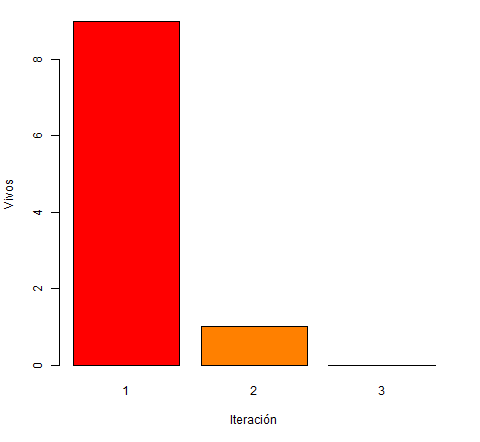
\includegraphics[width=\linewidth]{prob0-1.png}
\caption{Probabilidad de 0.1}
\label{prob1}
\end{subfigure}
\begin{subfigure}[b]{0.4\linewidth}
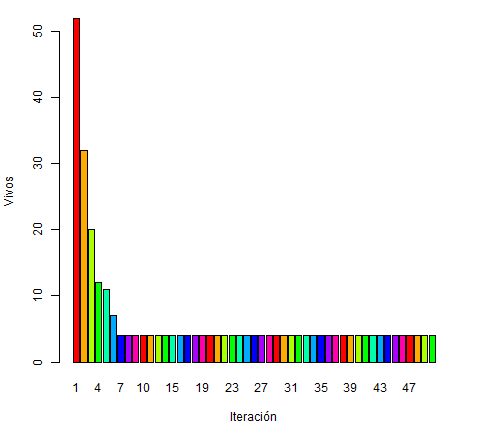
\includegraphics[width=\linewidth]{prob0-2.png}
\caption{Probabilidad de 0.2}
\label{prob2}
\end{subfigure}
\begin{subfigure}[b]{0.4\linewidth}
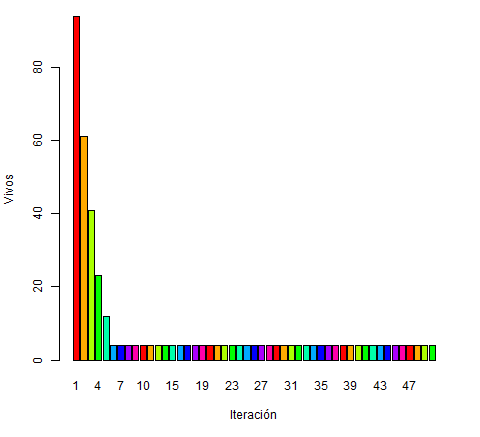
\includegraphics[width=\linewidth]{prob0-3.png}
\caption{Probabilidad de 0.3}
\label{prob3}
\end{subfigure}
\begin{subfigure}[b]{0.4\linewidth}
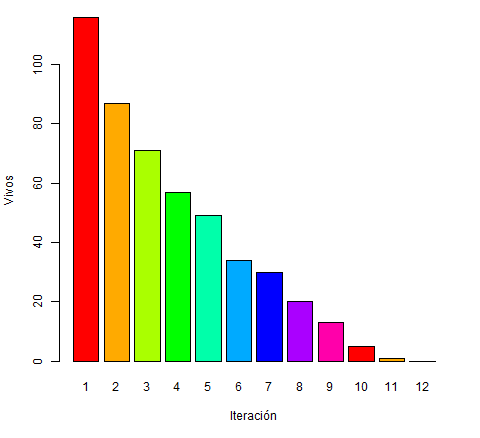
\includegraphics[width=\linewidth]{prob0-4.png}
\caption{Probabilidad de 0.4}
\label{prob4}
\end{subfigure}
\begin{subfigure}[b]{0.4\linewidth}
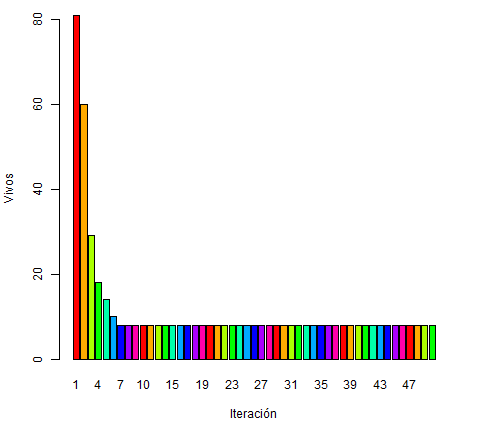
\includegraphics[width=\linewidth]{prob0-5.png}
\caption{Probabilidad de 0.5}
\label{prob5}
\end{subfigure}
\begin{subfigure}[b]{0.4\linewidth}
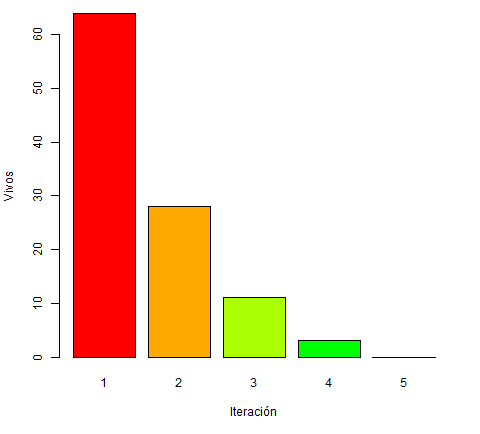
\includegraphics[width=\linewidth]{prob0-6.png}
\caption{Probabilidad de 0.6}
\label{prob6}
\end{subfigure}
\begin{subfigure}[b]{0.4\linewidth}
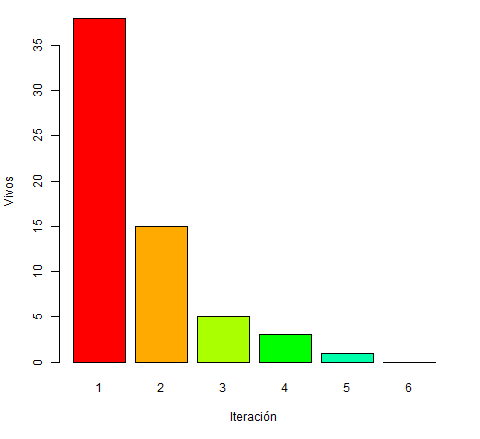
\includegraphics[width=\linewidth]{prob0-7.png}
\caption{Probabilidad de 0.7}
\label{prob7}
\end{subfigure}
\begin{subfigure}[b]{0.4\linewidth}
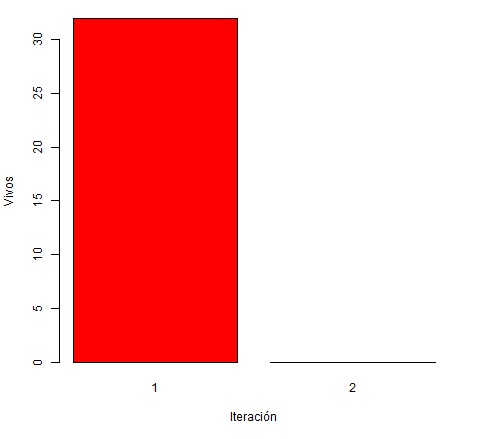
\includegraphics[width=\linewidth]{prob0-8.png}
\caption{Probabilidad de 0.8}
\label{prob8}
\end{subfigure}
\caption{Decremento en la población de celdas vivas por cada probabilidad inicial.}
\label{decremento}
\end{figure}

La tendencia general en todos los experimentos realizados es hacia un decremento en la población de celdas vivas, como se observa en la figura \ref{decremento}. Para las probabilidades de 0.1 y 0.8 el número de iteraciones es de tres y dos, respectivamente, ya  que la población culmina en cero rápidamente. En cuanto a las probabilidades de 0.4, 0.6 y 0.7, existe una mayor cantidad de iteraciones (doce, cinco y seis, respectivamente) antes de culminar en cero. 

Para las probabilidades de 0.2 y 0.3, el decremento jamás culmina en cero, sino en cuatro celdas vivas cuya posición influye en la supervivencia mutua para la siguiente iteración, por lo que el experimento se termina a las 50 repeticiones. Lo mismo se presenta en la probabilidad de 0.5, pero con la cantidad de ocho celdas vivas supervivientes.

\section{Conclusión}
La tendencia general de todos los experimentos es hacia un decremento poblacional, en donde el mayor colapso poblacional en celdas que mueren se presenta en casi todos los experimentos entre las primeras dos iteraciones.

\bibliography{P2}
\bibliographystyle{unsrtnat}

\end{document}